\chapter{Data: real recordings and synthetic generator}
\label{chap:data}

This chapter describes the real-world data on which the project is
grounded (\cref{sec:real-data}), the statistical model fitted to it
(\cref{sec:noise-model}), the parameterised anomaly templates that
encode the radiological events we want to learn (\cref{sec:templates}),
and the generator that combines these ingredients into a large labelled
training corpus (\cref{sec:generator}).

\section{Real 2015 gamma dose data}
\label{sec:real-data}

\subsection{Source}

The reference recordings are four months of gamma dose measurements
collected in 2015 by an environmental surveillance beacon and provided
by the project supervisor. The dates are
\begin{center}
\texttt{24/02/2015 11:20} \quad \texttt{30/04/2015 13:10} \quad
\texttt{22/06/2015 07:31} \quad \texttt{20/10/2015 09:18},
\end{center}
each segment lasting approximately $40\,000$ minutes (about $28$ days)
at one sample per minute. The four months are stored as separate
columns in a single text file under
\texttt{data-gen/data/}\,.

\begin{figure}[H]
    \centering
    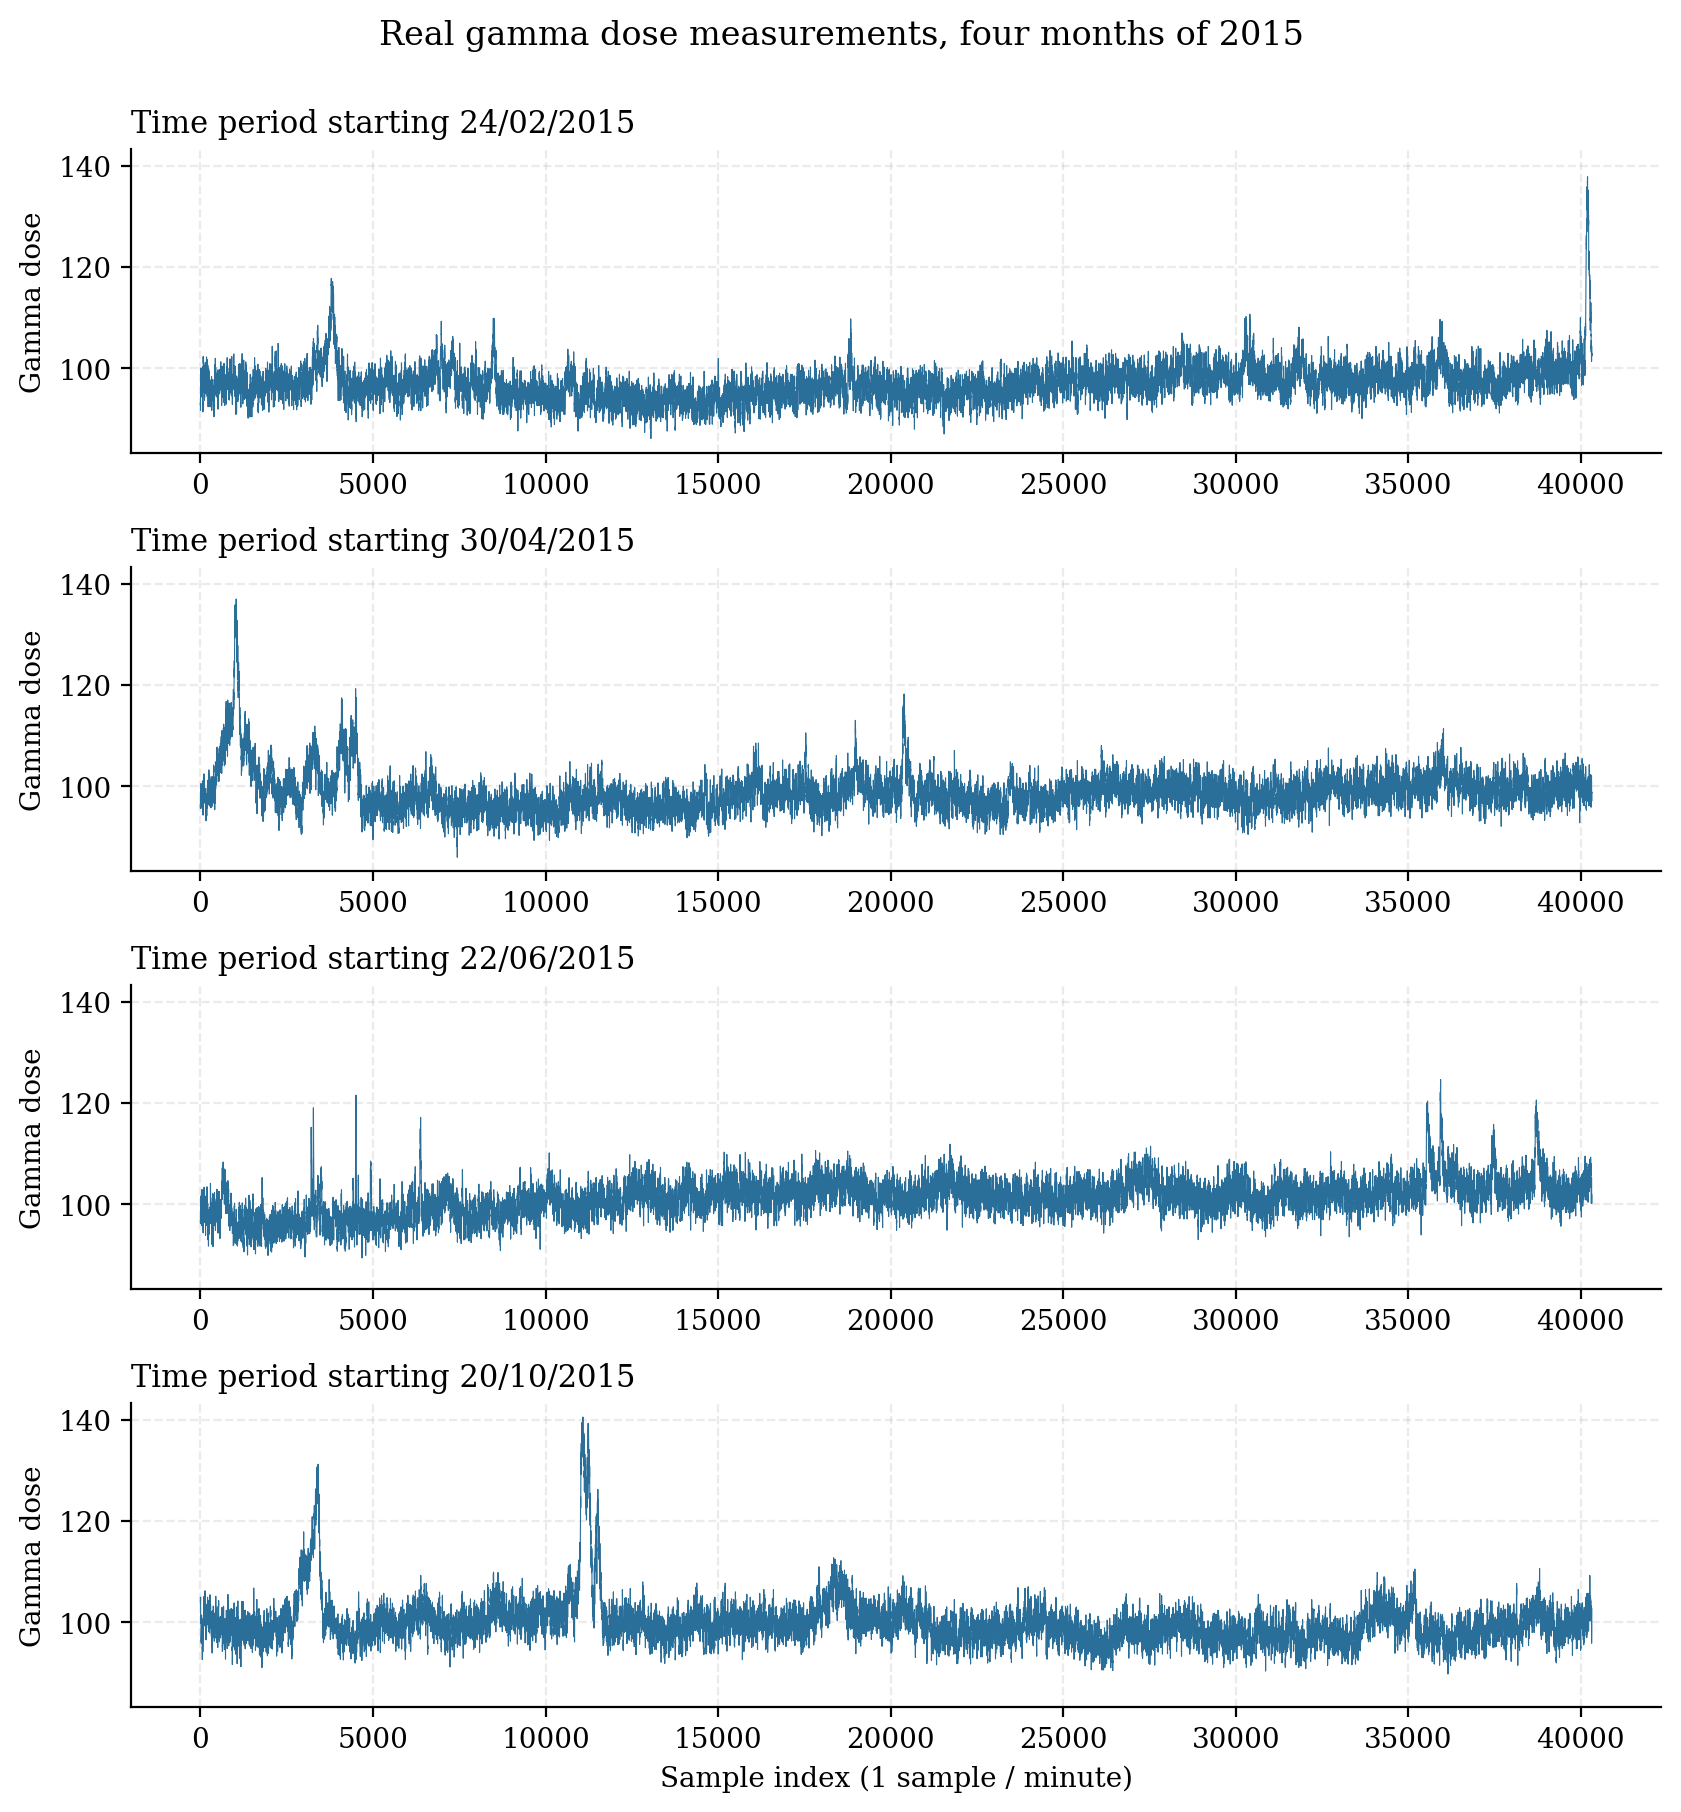
\includegraphics[width=0.85\linewidth]{figures/real_data_overview}
    \caption{The four months of real gamma-dose recordings provided by
    the supervisor. Each panel shows a continuous segment of
    approximately one month at one sample per minute. The signal is
    centred around $\sim 99$ counts with a high-frequency dispersion of
    a few counts and slow drifts of a few units; a small number of
    sharper excursions are visible (the spike near sample 38\,000 on
    February, the brief peak around sample 11\,000 on October).}
    \label{fig:real-overview}
\end{figure}

\subsection{Statistical characterisation}
\label{sec:stat-charac}

\Cref{fig:real-overview} suggests that the signal is the superposition
of (i) a slowly-varying baseline and (ii) a high-frequency,
zero-mean fluctuation. We confirm this by decomposing each month
with a moving-average estimator of window length $w = 480$ samples
(\cref{fig:real-decomp}):
\begin{equation}
    b_t = \frac{1}{w} \sum_{i = -w/2}^{w/2} x_{t+i},
    \qquad r_t = x_t - b_t.
\end{equation}

\begin{figure}[H]
    \centering
    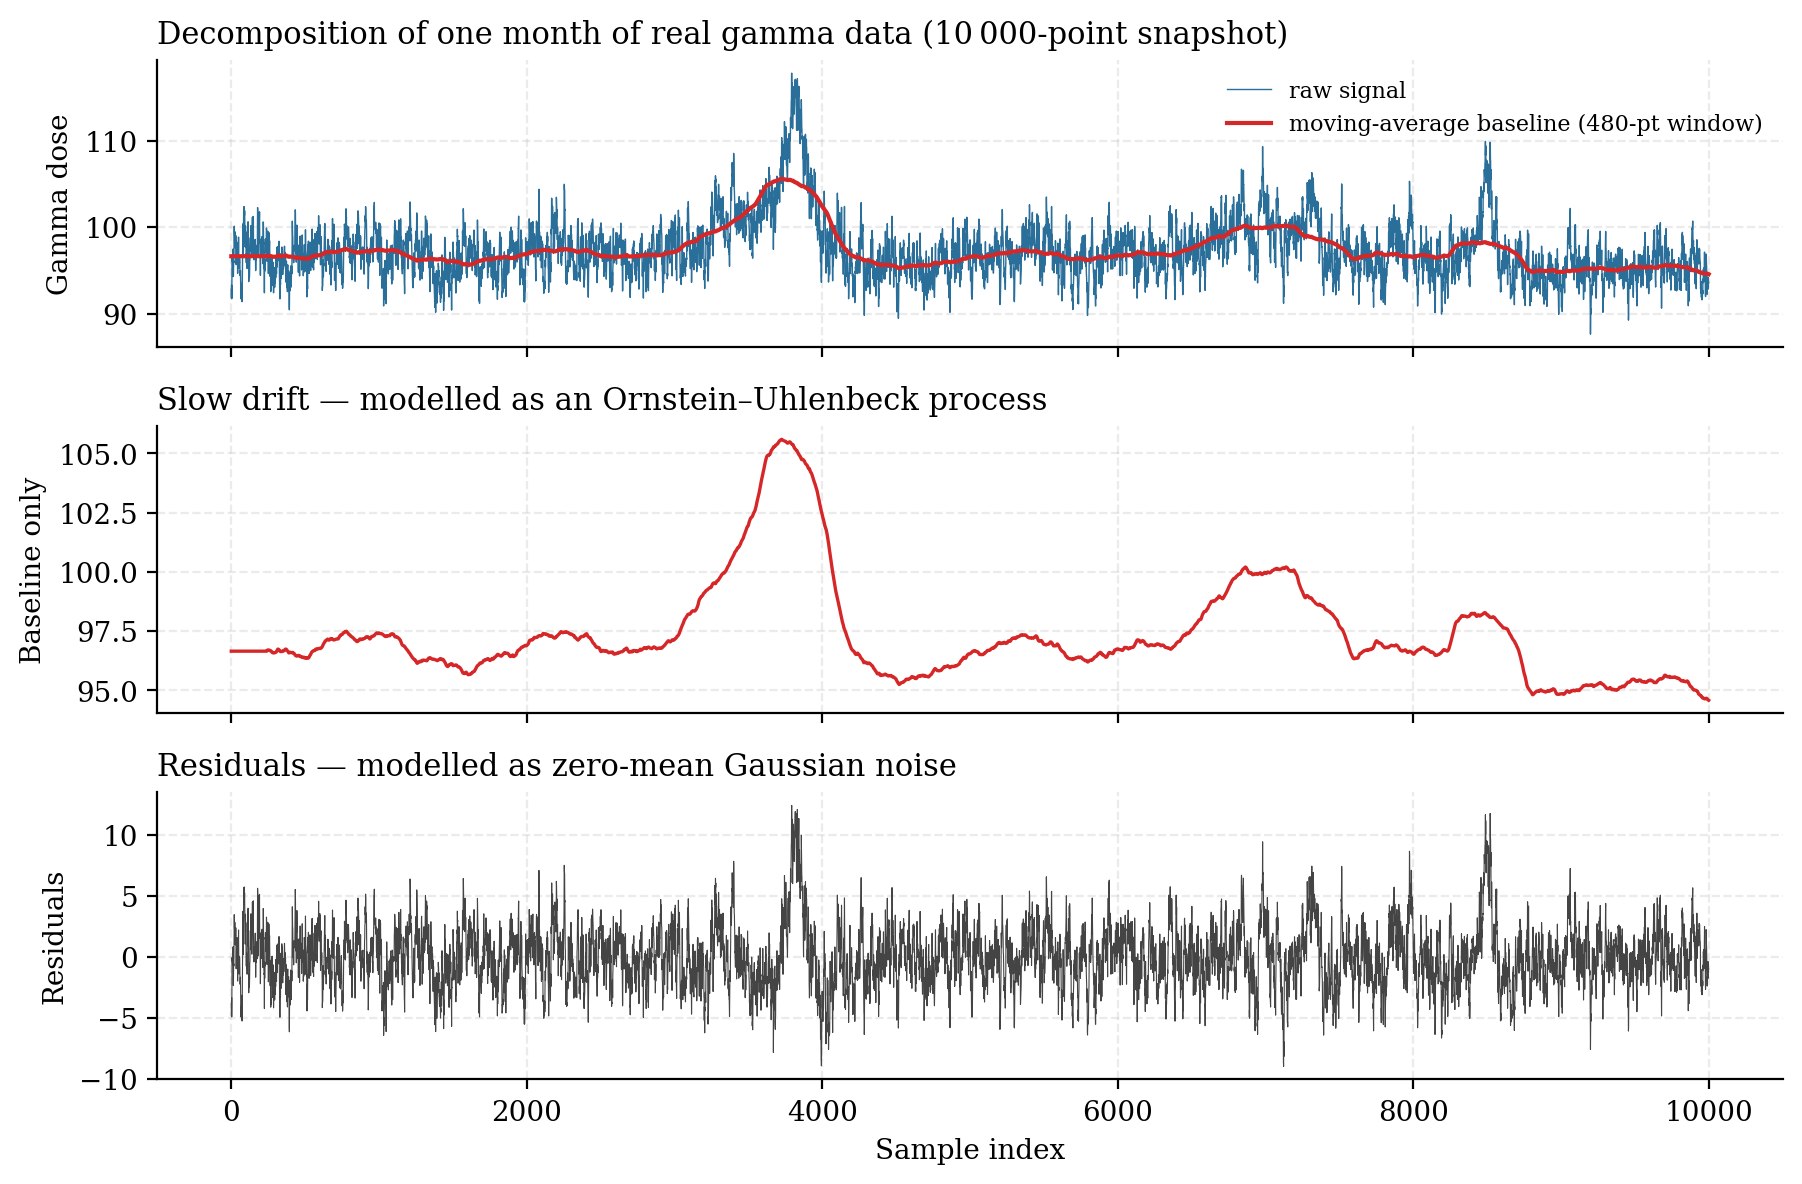
\includegraphics[width=0.95\linewidth]{figures/real_data_decomposition}
    \caption{Decomposition of a $10\,000$-sample snapshot of the first
    month of real data into a slowly-varying baseline (red) and
    zero-mean residuals (bottom). The baseline is computed as a
    centred moving average with a $w=480$-sample window. The residuals
    look stationary, zero-mean, and approximately Gaussian.}
    \label{fig:real-decomp}
\end{figure}

The empirical statistics, averaged across the four months, are reported
in \cref{tab:real-stats}. The baseline standard deviation is much
smaller than the high-frequency residual standard deviation, but its
\emph{slow} variation is what motivates the random-walk baseline model
used in the synthetic generator.

\begin{table}[H]
    \centering
    \footnotesize
    \begin{tabular}{lcccc}
        \toprule
        Month & Global mean $\mu$ & HF noise std $\sigma$ & OU $\theta$ & OU $\sigma_{\mathrm{OU}}$ \\
        \midrule
        24/02/2015 & 96.93  & 2.31 & $4 \cdot 10^{-6}$ & 0.0277 \\
        30/04/2015 & 98.86  & 2.58 & $4 \cdot 10^{-6}$ & 0.0390 \\
        22/06/2015 & 101.28 & 2.51 & $4 \cdot 10^{-6}$ & 0.0337 \\
        20/10/2015 & 99.95  & 2.70 & $4 \cdot 10^{-6}$ & 0.0485 \\
        \midrule
        \textbf{Average across all} & \textbf{99.26} & \textbf{2.53} & $\mathbf{4 \cdot 10^{-6}}$ & \textbf{0.0373} \\
        \bottomrule
    \end{tabular}
    \caption{Statistical characterisation of the four months of real
    gamma data, as extracted by \texttt{data-gen/evaluate\_real\_data.py}.
    The averaged values in the bottom row are those used in the
    synthetic generator.}
    \label{tab:real-stats}
\end{table}

\begin{figure}[H]
    \centering
    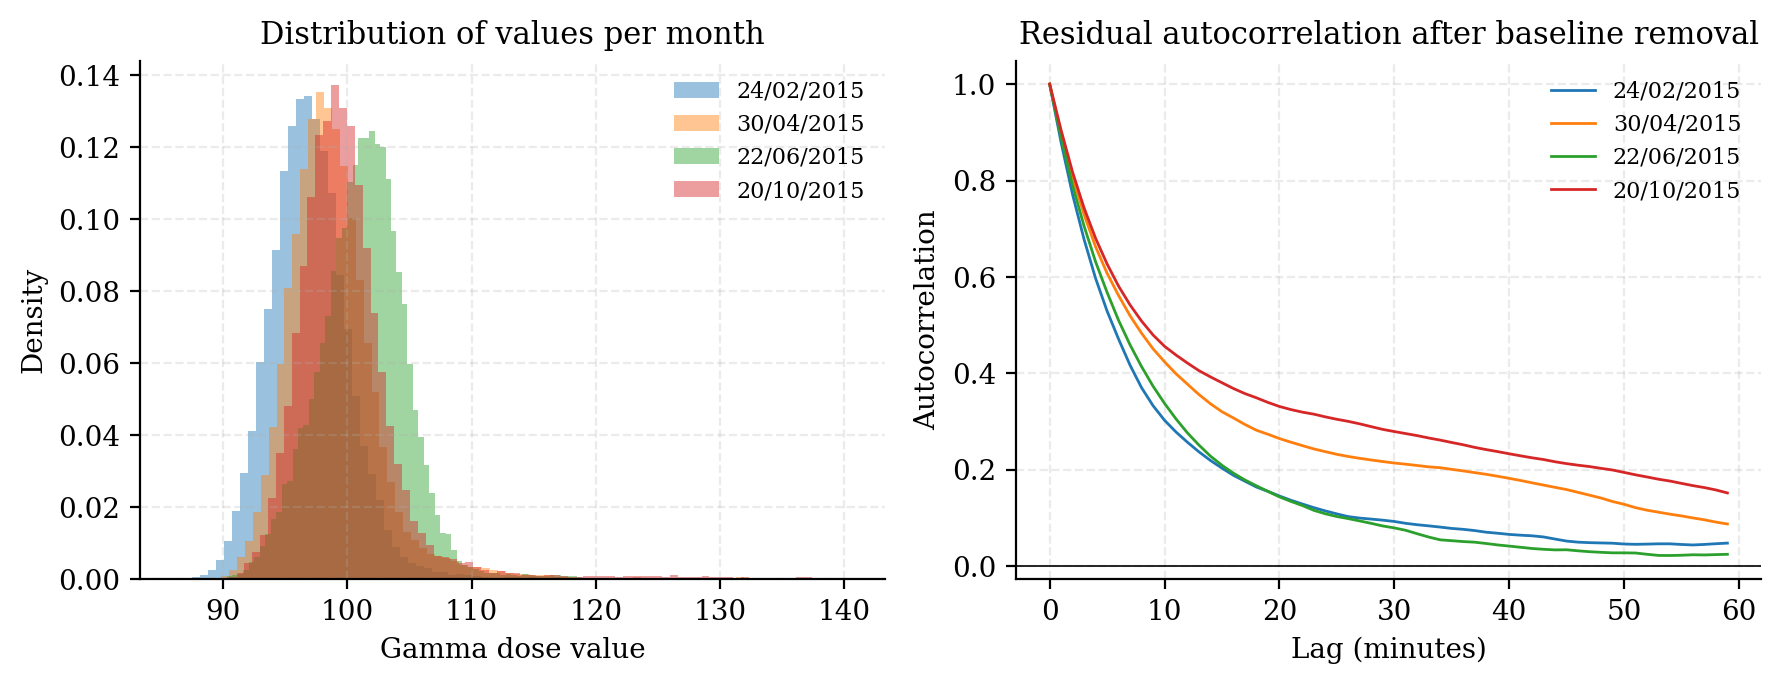
\includegraphics[width=0.95\linewidth]{figures/real_data_stats}
    \caption{Left: empirical distribution of the raw gamma dose values
    per month. The distributions are unimodal and only slightly
    skewed, supporting a Gaussian approximation of the high-frequency
    noise. Right: autocorrelation of the residuals (after baseline
    removal) decays rapidly; remaining short-lag correlation indicates
    that the moving-average filter still leaks a small amount of
    drift into the residuals.}
    \label{fig:real-stats}
\end{figure}

\section{Noise model: Gaussian fluctuations on an OU baseline}
\label{sec:noise-model}

Following the empirical findings of \cref{sec:stat-charac}, we model
the real gamma dose as
\begin{equation}
    x_t = b_t + \eta_t,
    \quad \eta_t \overset{\text{iid}}{\sim} \mathcal{N}(0, \sigma^2),
    \quad b_{t+1} = b_t + \theta (\mu - b_t) + \xi_t,
    \quad \xi_t \overset{\text{iid}}{\sim} \mathcal{N}(0, \sigma_{\mathrm{OU}}^2).
    \label{eq:noise-model}
\end{equation}
The first equation says that the instantaneous reading is a baseline
plus zero-mean Gaussian noise; the second is the Ornstein--Uhlenbeck
(OU) discrete dynamics for the baseline. The parameter $\theta$
controls the mean-reversion strength: $b_t$ is pulled towards the
long-run mean $\mu$ at a rate $\theta$, with random kicks of magnitude
$\sigma_{\mathrm{OU}}$. With $\theta=4 \cdot 10^{-6}$, the baseline is
very loosely tethered: the half-life of an excursion is roughly
$\log 2 / \theta \approx 1.7 \cdot 10^{5}$ samples, much longer than
our analysis windows. This reproduces the slow drifts visible in
\cref{fig:real-overview}.

\section{Anomaly templates}
\label{sec:templates}

The six anomaly classes are described as \emph{piecewise-interpolated
parametric curves} stored as small CSV files in
\texttt{data-gen/anomalies/}. Each row defines a \emph{keypoint} with
six fields plus an interpolation flag:
\begin{itemize}[leftmargin=*, itemsep=0.2em]
    \item \texttt{time} $\in [0,1]$, \texttt{value} $\in [0,1]$ ---
    the position of the keypoint in normalised time and amplitude;
    \item \texttt{t\_minus, t\_plus, v\_minus, v\_plus} $\in \{0, 1\}$
    --- boolean flags that mark which quadrants the keypoint is
    allowed to move into when the template is jittered;
    \item \texttt{interp} $\in \{\texttt{linear}, \texttt{exp\_up},
    \texttt{exp\_down}, \texttt{bell}\}$ --- the interpolation mode for
    the segment that starts at this keypoint.
\end{itemize}

\Cref{fig:templates} shows the six clean templates. Visually, they
correspond to four common families of radiological signatures:
\begin{itemize}[leftmargin=*, itemsep=0.2em]
    \item \textbf{Smooth bumps} (\texttt{bell}, \texttt{bell\_sq}):
    plumes that build up and decay smoothly, possibly with a small
    sustained plateau.
    \item \textbf{Asymmetric ramps} (\texttt{fast\_ascend},
    \texttt{fast\_descend}): rapid onset followed by slow exponential
    decay, or its time-reverse.
    \item \textbf{Plateau} (\texttt{square}): a sustained
    contamination episode.
    \item \textbf{Multi-peak} (\texttt{M}): two close consecutive
    events --- a useful adversarial shape for the network.
\end{itemize}

\begin{figure}[H]
    \centering
    
\includegraphics[width=0.95\linewidth]{figures/anomaly_templates}
    \caption{The six hand-designed anomaly templates, drawn in
    normalised time and amplitude. Each template is encoded as a small
    list of keypoints (red dots) connected by linear, exponential or
    half-cosine (``bell'') segments.}
    \label{fig:templates}
\end{figure}

\subsection{Stochastic deformation of a template}
\label{sec:deformation}

A template would be useless on its own --- training a network to
recognise the exact same shape would not generalise. We therefore
\emph{deform} each template before injecting it into the signal. The
algorithm, implemented in \texttt{anomaly\_generator.py}, perturbs
each keypoint independently by an isotropic Gaussian jitter of
standard deviation $\nu$ (the \emph{variance level}), then enforces
the direction constraints encoded by the \texttt{t\_minus}, \dots,
\texttt{v\_plus} flags so that the deformed template still has the
right qualitative shape (a peak cannot become a valley, time monotonicity
is enforced as a fail-safe). The resulting deformed keypoints are then
interpolated back into a dense curve and re-scaled to the target
amplitude and period:
\begin{equation}
    \text{amplitude} \in \sigma \cdot [\,2.5,\, 7.6\,],
    \qquad
    \text{period} \in [200,\, 800] \text{ samples},
    \qquad
    \nu \in [0.02,\, 0.10].
\end{equation}
The amplitude is expressed in multiples of the high-frequency noise
standard deviation $\sigma$, so that the per-sample signal-to-noise
ratio of a generated anomaly lies in the interesting range
$[2.5, 7.6]$.

\begin{figure}[H]
    \centering
    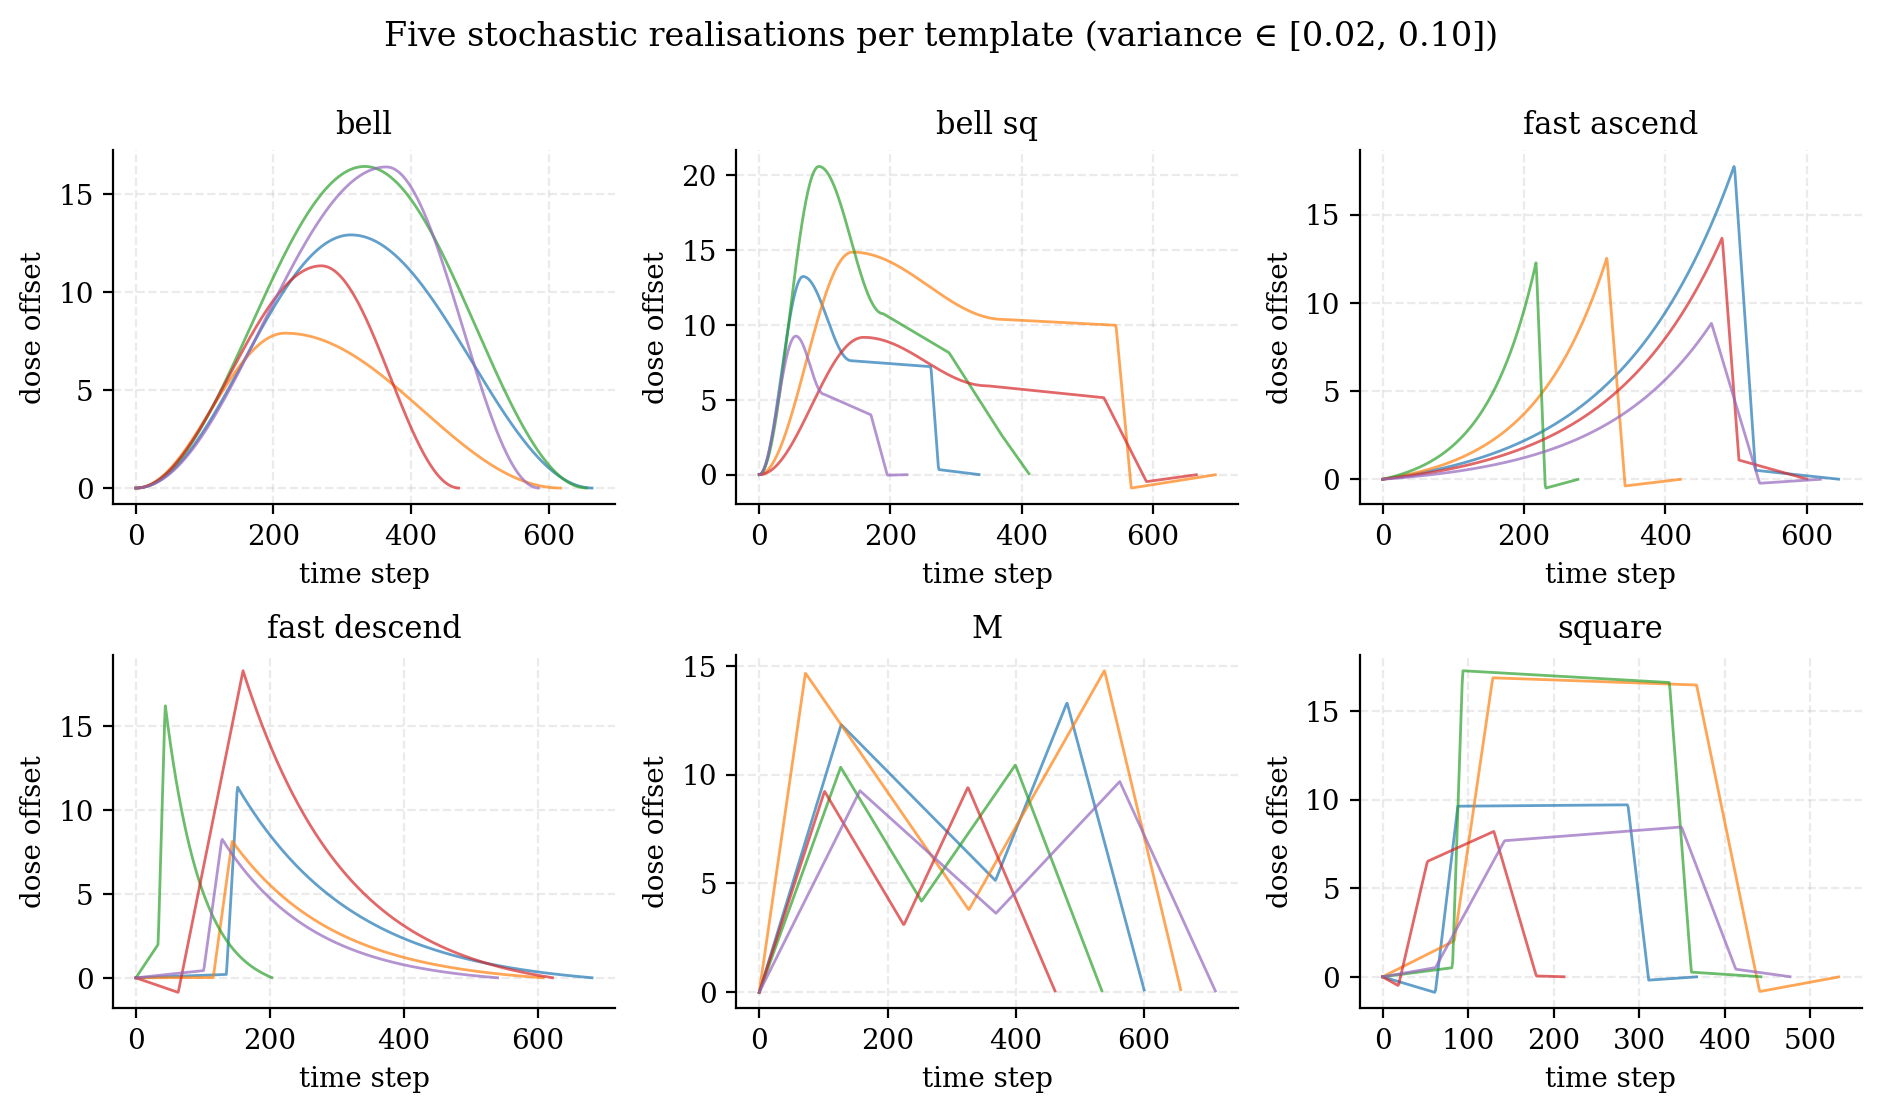
\includegraphics[width=0.95\linewidth]{figures/template_deformation}
    \caption{Five stochastic realisations of each template with random
    amplitude, period and deformation variance in the ranges used at
    training time. The qualitative shape is preserved, but no two
    realisations are identical.}
    \label{fig:deformation}
\end{figure}

\section{Synthetic data generator}
\label{sec:generator}

The end-to-end generator (\texttt{generate\_custom\_dataset.py})
combines the noise model of \cref{sec:noise-model} and the deformed
templates of \cref{sec:deformation} into a long labelled signal.

\subsection{Algorithm}
\label{sec:gen-algo}

In pseudo-code, generating $N$ points proceeds as follows:
\begin{enumerate}[leftmargin=*, itemsep=0.2em]
    \item Pick the total number of anomalies $M \in [5\,000, 8\,000]$ and
    pre-compute their evenly-spaced injection indices, with a small
    random jitter ($\pm 200$ samples) around each grid point.
    \item For each injection point, sample a template uniformly at
    random, sample $(\text{amplitude}, \text{period}, \nu)$ from their
    ranges, and produce the deformed dense curve.
    \item Generate the background in $50\,000$-point chunks: simulate the
    OU baseline path and overlay $\mathcal{N}(b_t, \sigma^2)$ noise.
    \item Add each anomaly curve on top of the background at its
    injection index and label every output point with the anomaly's
    class (or $0$ if the per-point contribution falls below a small
    threshold $10^{-2}$).
\end{enumerate}

The final dataset is written to disk in CSV chunks; it never lives
entirely in RAM, which lets us produce datasets of arbitrary size
within a constant memory budget.

\subsection{Dataset used for this report}
\label{sec:final-dataset}

For this report we generate $N = 10^{7}$ samples and inject in the
range $[5\,000, 8\,000]$ anomalies, leading to a global anomaly density
of $\sim 7$ events per $10\,000$ samples. The signal looks as in
\cref{fig:synth-preview}.

\begin{figure}[H]
    \centering
    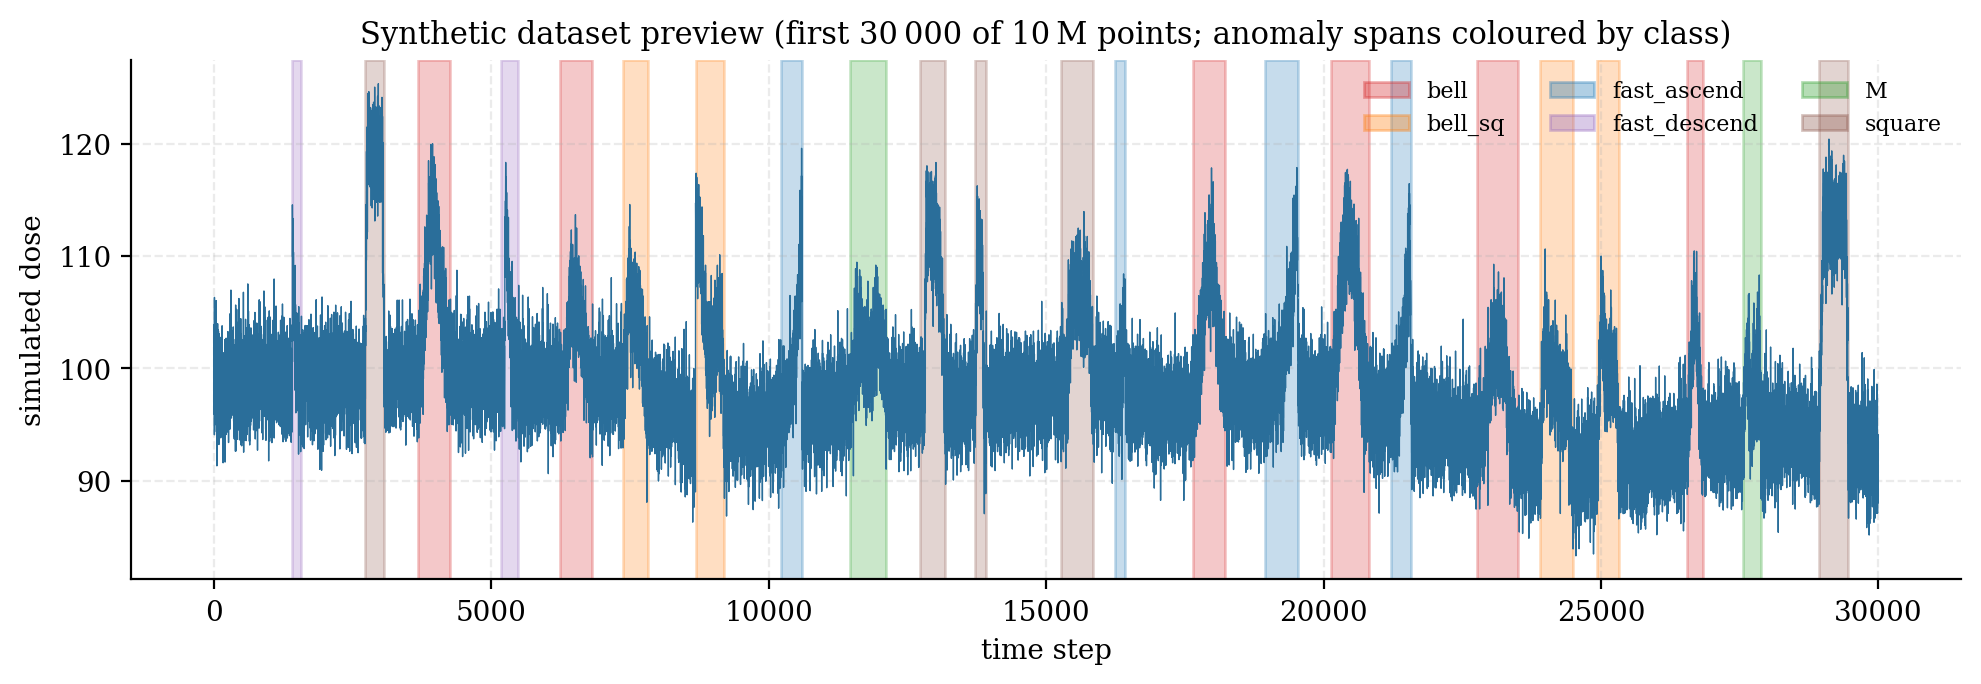
\includegraphics[width=\linewidth]{figures/synthetic_dataset_preview}
    \caption{First $30\,000$ samples (of $10^{7}$) of the generated
    synthetic dataset. Anomaly spans are coloured by class. The
    background standard deviation matches the real data of
    \cref{tab:real-stats}; anomaly densities are deliberately higher
    than in the real recordings, so that the model is exposed to many
    examples of each class.}
    \label{fig:synth-preview}
\end{figure}

\subsection{Why \emph{this} generator?}

Two design choices deserve a quick comment, because they will resurface
in \cref{chap:realdata}.

\paragraph{Anomaly density is much higher than the real world.} The
synthetic dataset contains roughly one anomaly every $1\,500$ samples,
whereas the real recordings contain a handful of plausible anomalies
over $40\,000$ samples. This is a deliberate choice to give the
classifier many examples of each class, but it skews the class prior
seen by the network. We will see in \cref{sec:fail-prior} that this is
the largest single contributor to the model's failure on real data.

\paragraph{Templates assume a clear anomaly shape.} The generator
produces anomalies that are clean, isolated, and have a well-defined
duration in $[200, 800]$ samples. Real-life events may be much shorter
(a single contaminated sample) or much longer (a contamination episode
that lasts hours), and the recordings also contain rapid, isolated
single-point excursions that the templates do not represent at all. The
trained classifier is therefore intrinsically blind to these
out-of-template events.
